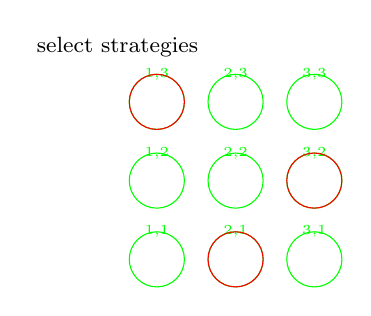
\begin{tikzpicture}
    %\draw[thin, dashed] (0, 0) rectangle (3, 3);
    \foreach \x in {1, 2, 3}
        \foreach \y in {1, 2, 3}
            {\draw[green] (\x-0.5, \y-0.5) circle (0.35);
            \node[green] at (\x-0.5, \y-0.15) {\tiny \x,\y};}
    \node at (0, 3.2) {\footnotesize select strategies};
    \draw[red] (1-0.5, 3-0.5) circle (0.35);
    \draw[red] (2-0.5, 1-0.5) circle (0.35);
    \draw[red] (3-0.5, 2-0.5) circle (0.35);
\end{tikzpicture}